\documentclass[11pt,a4paper]{article}
% Preambulo comun de los reportes de Tecnologias Celulares.
% Cada main.tex hace: \documentclass ... \input{../comun/preambulo.tex}
\usepackage[utf8]{inputenc}
\usepackage[T1]{fontenc}
\usepackage[spanish,mexico]{babel}
\usepackage{graphicx}
\usepackage[margin=2.5cm]{geometry}
\usepackage{amsmath}
\usepackage{amssymb}
\usepackage{booktabs}
\usepackage{tabularx}
\usepackage{array}
\usepackage{float}
\usepackage{setspace}
\usepackage{parskip}
\usepackage{fancyhdr}
\usepackage{textcomp}
\usepackage{xcolor}
\usepackage{caption}
\usepackage{fvextra}
\usepackage[hidelinks]{hyperref}

\onehalfspacing
\setlength{\parskip}{6pt}
\sloppy
\setlength{\emergencystretch}{3em}
\setlength{\headheight}{40pt}
\captionsetup{font=small,labelfont=bf}
\setlength{\tabcolsep}{6pt}

\pagestyle{fancy}
\fancyhf{}
\fancyhead[L]{\includegraphics[width=1cm]{/home/yovick/repos/UAZ-IEI/Assets/UIE.png}}
\fancyhead[R]{\small Tecnologías Celulares}
\fancyfoot[C]{\thepage}
\renewcommand{\headrulewidth}{0.4pt}

\DefineVerbatimEnvironment{codigo}{Verbatim}{%
  breaklines=true,breakanywhere=true,fontsize=\small,frame=single,
  framesep=3pt,rulecolor=\color{gray!50}}

% Figura centrada con pie: \figura[ancho]{archivo}{leyenda}
\newcommand{\figura}[3][0.85]{%
  \begin{center}
    \includegraphics[width=#1\linewidth]{#2}\\[2pt]
    {\small #3}
  \end{center}}

% Portada: \portada{numero}{titulo de la practica}
\newcommand{\portada}[2]{%
\begin{titlepage}
  \thispagestyle{empty}
  \begin{center}
    \vspace*{1cm}
    \includegraphics[width=4.5cm]{/home/yovick/repos/UAZ-IEI/Assets/uaz.png}
    \vspace{0.8cm}

    {\large Universidad Autónoma de Zacatecas}\\[4pt]
    {\large Unidad Académica de Ingeniería Eléctrica}\\[4pt]
    {\normalsize Ingeniería Electrónica Industrial con especialidad en Telecomunicaciones}

    \vspace{1.8cm}
    {\LARGE\bfseries Práctica #1}\\[10pt]
    {\Large\bfseries #2}
  \end{center}

  \vspace{2.2cm}
  \begin{center}
    \begin{tabular}{rl}
      \textbf{Materia:} & Tecnologías Celulares\\
      \textbf{Docente:} & Dr. Víktor Iván Rodríguez Abdalá\\
      \textbf{Alumno:}  & Arnold Yovick Ríos Zaldívar\\
      \textbf{Fecha:}   & Noviembre de 2026\\
    \end{tabular}
  \end{center}
  \vfill
\end{titlepage}}


\graphicspath{{figs/}}

% Listado leido del archivo real: el PDF siempre muestra el codigo que corrio.
\newcommand{\listado}[1]{%
  \VerbatimInput[fontsize=\scriptsize,breaklines=true,breakanywhere=true,
    frame=single,framesep=2pt,rulecolor=\color{gray!50},numbers=left,
    numbersep=4pt]{#1}}

\begin{document}
\thispagestyle{empty}

% --------------------------------------------------------------- encabezado
\begin{center}
  \includegraphics[width=2.6cm]{/home/yovick/repos/UAZ-IEI/Assets/uaz.png}\\[2mm]
  {\large Universidad Autónoma de Zacatecas}\\
  {\normalsize Unidad Académica de Ingeniería Eléctrica}\\
  {\normalsize Ingeniería Electrónica Industrial con especialidad en Telecomunicaciones}\\[6mm]
  {\LARGE\bfseries Tarea 3}\\[2mm]
  {\large OFDM: generación, ruido, espectro y PAPR}\\[5mm]
  {\small
  \begin{tabular}{rl}
    \textbf{Materia:}   & Tecnologías Celulares\\
    \textbf{Docente:}   & Dr. Víktor Iván Rodríguez Abdalá\\
    \textbf{Alumno:}    & Arnold Yovick Ríos Zaldívar\\
    \textbf{Matrícula:} & 35167151 \quad \textbf{Grupo:} VII\\
    \textbf{Fecha:}     & Noviembre de 2026\\
  \end{tabular}}
\end{center}

\vspace{2mm}

Los siete problemas se resolvieron con un solo script de Python,
\texttt{tarea3.py}, que genera las figuras y los números citados. Se usan
símbolos 4-PSK de energía unitaria (16-QAM en el problema 1), $K$ subportadoras y
$x[n]=\frac{1}{\sqrt N}\sum_k X_k e^{j2\pi kn/N}$ (IFFT); para la PAPR se usa
la forma real $x(t)=\sum_k \cos(2\pi kt/T+\theta_k)$ con 200 muestras por
símbolo. Todo se regenera con \texttt{python3 tarea3.py}.

% ------------------------------------------------------------- problema 1
\section{Problema 1: cuatro símbolos 16-QAM}

Se repite el problema ilustrativo 2 con cuatro símbolos 16-QAM. Con $K=5$ y
$N=10$, el espectro hermítico
$[0,\ X_1,\dots,X_4,\ 0,\ X_4^*,\dots,X_1^*]$ hace que $x(t)$ sea real. La
figura compara $x(t)$ con las muestras $x(nT/N)$: el error máximo es
$6.9\times10^{-15}$. La FFT recupera los cuatro símbolos con error
$5.6\times10^{-16}$.

\begin{figure}[H]
  \centering
  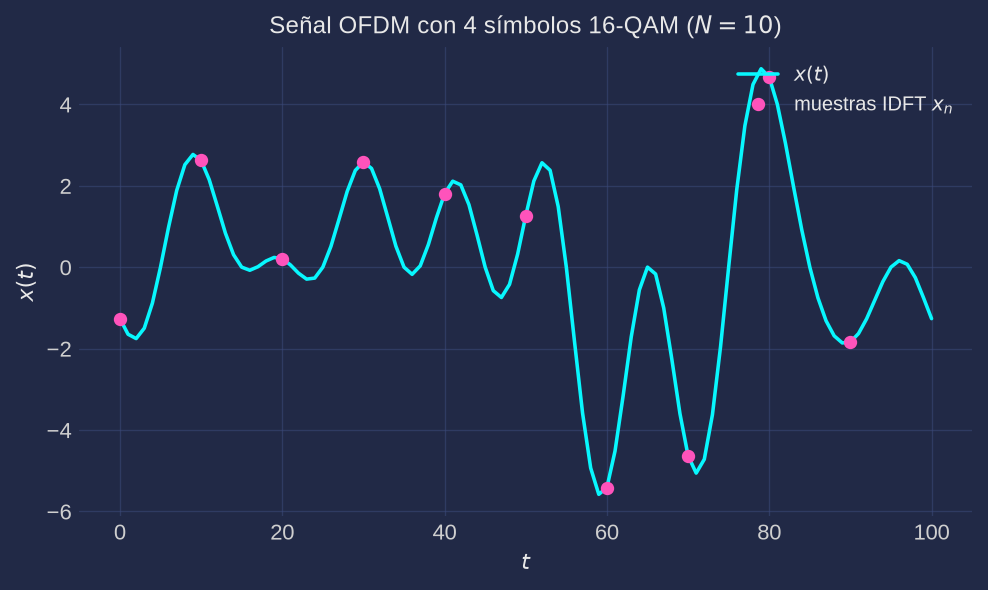
\includegraphics[width=0.66\linewidth]{p1_senal.png}
  \caption{Señal OFDM de 4 símbolos 16-QAM y sus muestras IDFT.}
\end{figure}

% ------------------------------------------------------------- problema 2
\section{Problema 2: 4-PSK con $K=16$ y FFT}

Se generan 16 símbolos 4-PSK y se sintetiza el símbolo con
$x=\sqrt K\,\mathrm{IFFT}(X)$. La FFT recupera los 16 símbolos con error
$2.2\times10^{-16}$ y la constelación cae en $\pm1\pm j$ sobre $\sqrt2$, como
muestra la figura.

\begin{figure}[H]
  \centering
  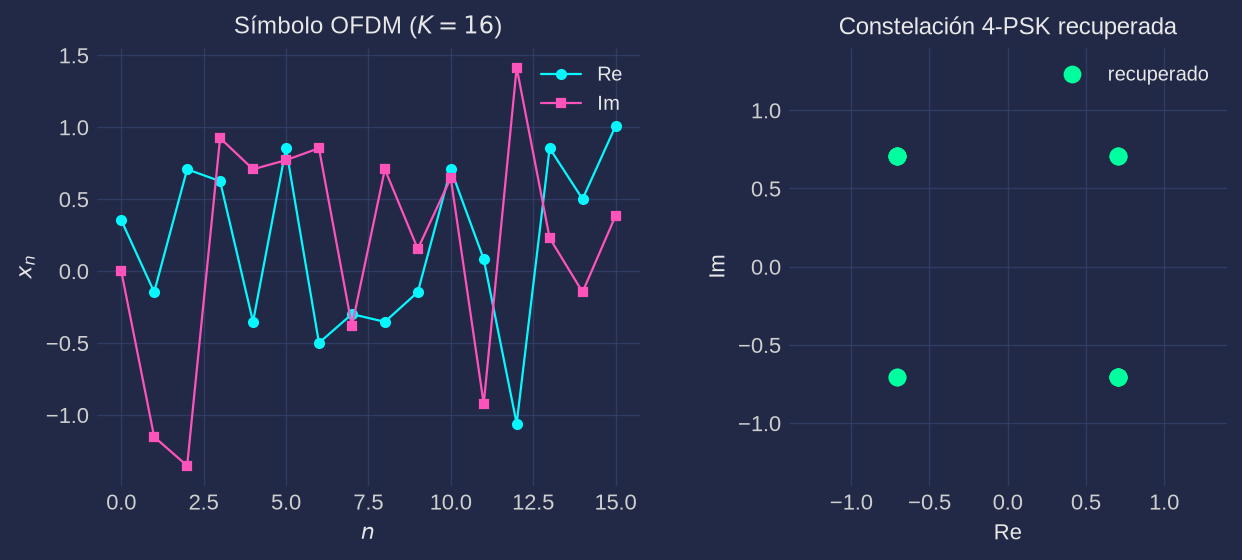
\includegraphics[width=0.9\linewidth]{p2_simbolo.png}
  \caption{Símbolo OFDM de 16 subportadoras y constelación recuperada.}
\end{figure}

% ------------------------------------------------------------- problema 3
\section{Problema 3: ruido aditivo}

Se suma ruido gaussiano complejo de varianza $\sigma^2$ a las muestras y se
demodula con la FFT; el detector elige el punto 4-PSK más cercano. Para una
realización con $\sigma^2=1,2,4$ se detectaron 5, 8 y 9 errores de 16. Sobre
4000 símbolos, la SER medida es 4.5\%, 14.7\%, 29.3\%, 42.5\% y 52.6\% para
$\sigma^2=0.25,0.5,1,2,4$: el enlace es usable hasta $\sigma^2\approx0.25$ y
con $\sigma^2\ge2$ el ruido domina.

\begin{figure}[H]
  \centering
  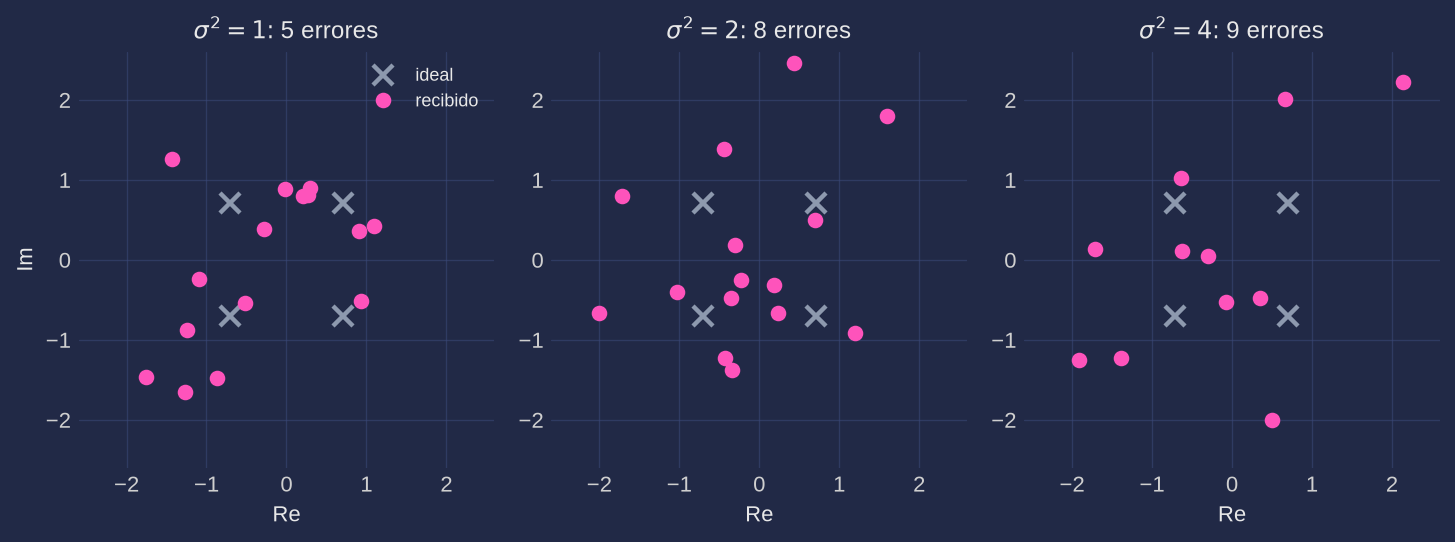
\includegraphics[width=\linewidth]{p3_ruido.png}
  \caption{Constelaciones recibidas para $\sigma^2=1,2,4$ (cruz: ideal;
  punto: recibido).}
\end{figure}

% ------------------------------------------------------------- problema 4
\section{Problema 4: espectro de la señal OFDM}

La transformada de $x(t)$ es
\begin{equation}
  X(f)=\sqrt T\sum_{k=0}^{K-1}X_k\,e^{-j\pi(fT-k)}\,
  \operatorname{sinc}(fT-k),
\end{equation}
una suma de lóbulos sinc centrados en $k/T$. La figura muestra $|X(f)|$ en dB
para $K=16$; el máximo entre portadoras es 3.65 dB. La FFT con relleno de ceros
(16384 puntos) reproduce la curva analítica.

\begin{figure}[H]
  \centering
  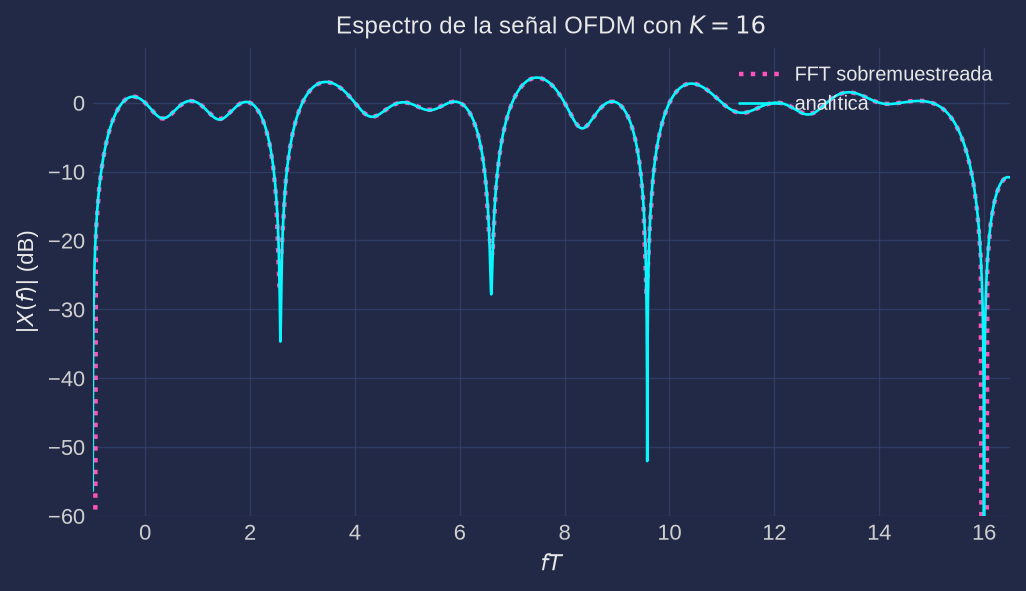
\includegraphics[width=0.82\linewidth]{p4_espectro.png}
  \caption{Espectro de la señal OFDM: expresión analítica y verificación por
  FFT.}
\end{figure}

% ------------------------------------------------------------- problema 5
\section{Problema 5: PAPR con $K=16$}

Se calculó la PAPR de 1000 realizaciones,
$\mathrm{PAPR}=\max|x|^2/\mathrm{E}\{|x|^2\}$, con $K=16$ y fases 4-PSK. La
media es 8.39 dB, la desviación 1.12 dB y el máximo 12.32 dB; el 1\% de las
realizaciones supera 11.5 dB.

\begin{figure}[H]
  \centering
  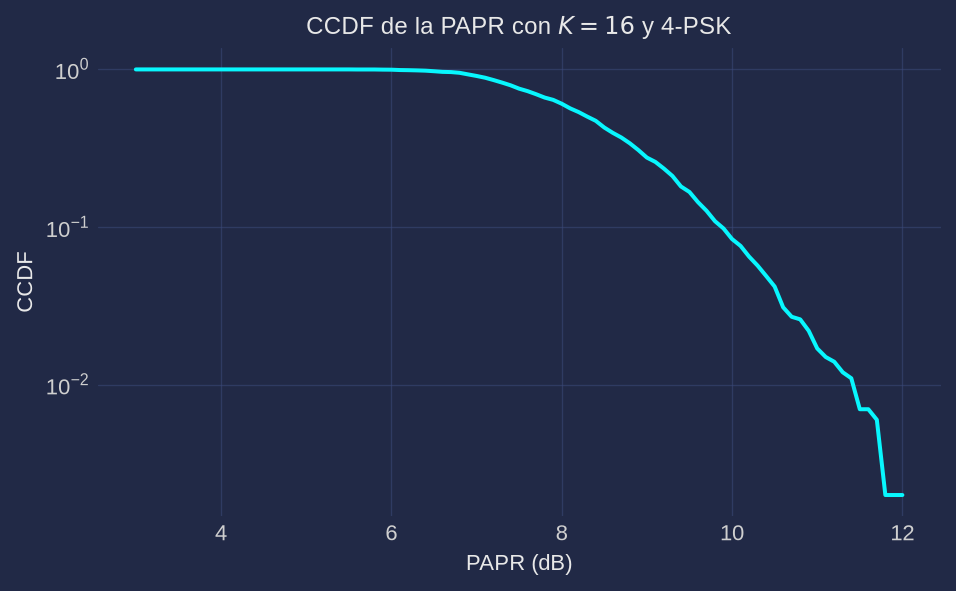
\includegraphics[width=0.65\linewidth]{p5_papr.png}
  \caption{CCDF de la PAPR para $K=16$.}
\end{figure}

% ------------------------------------------------------------- problema 6
\section{Problema 6: recorte de picos a 4 y 6 dB}

Se aplicó un recorte iterativo de amplitud hasta garantizar
$\mathrm{PAPR}\le4$ dB y $\le6$ dB. La PAPR queda exactamente en el umbral en
todas las realizaciones. El costo es distorsión: el EVM medio es 25.3\% a
4 dB y 10.5\% a 6 dB. Recortar a 6 dB es un compromiso razonable; a 4 dB la
señal se deforma visiblemente.

\begin{figure}[H]
  \centering
  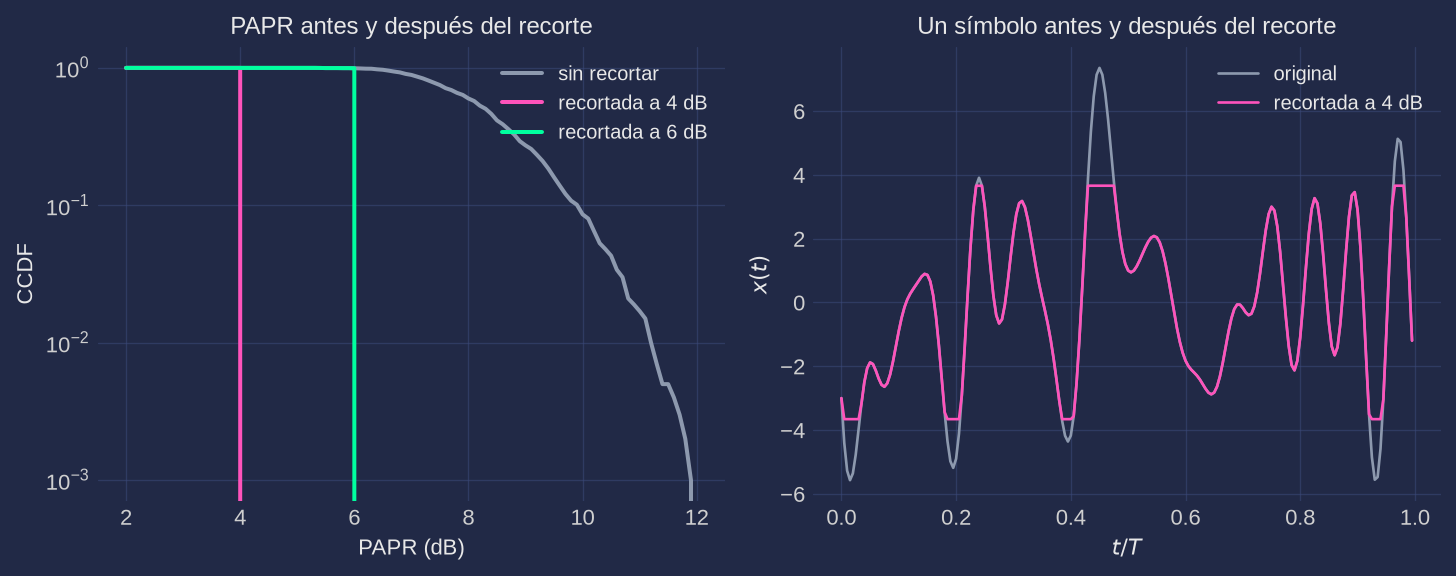
\includegraphics[width=\linewidth]{p6_recorte.png}
  \caption{PAPR antes y después del recorte (izquierda) y efecto del recorte
  sobre un símbolo (derecha).}
\end{figure}

% ------------------------------------------------------------- problema 7
\section{Problema 7: SLM con $K=8$}

Se repitió el método de fase aleatoria con $K=8$, $M=4$ candidatos y 4-PSK. La
PAPR media baja de 7.45 a 6.29 dB (1.17 dB de mejora) y la CCDF se desplaza a
la izquierda. El receptor necesita conocer el vector de fases elegido.

\begin{figure}[H]
  \centering
  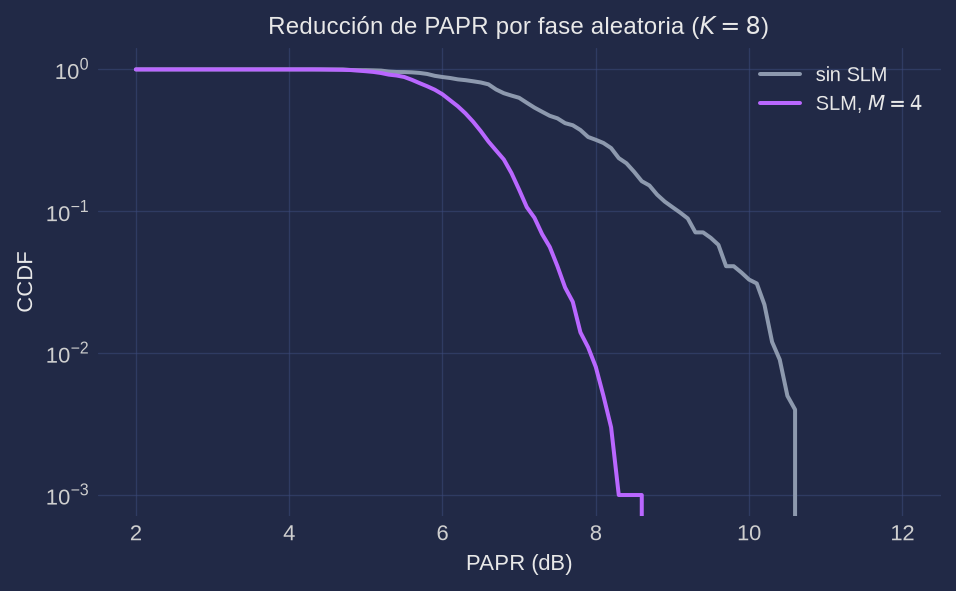
\includegraphics[width=0.65\linewidth]{p7_slm.png}
  \caption{CCDF de la PAPR con y sin SLM para $K=8$.}
\end{figure}

% ------------------------------------------------------------- conclusiones
\section{Conclusiones}

\begin{itemize}
  \item La IDFT/FFT reproduce la señal y recupera los símbolos con error de
        máquina ($\sim10^{-15}$).
  \item El ruido degrada la constelación de forma monótona: la SER pasa de
        4.5\% a 52.6\% al crecer $\sigma^2$ de 0.25 a 4.
  \item El espectro de OFDM es una suma de lóbulos sinc; la FFT con relleno de
        ceros valida la expresión analítica.
  \item La PAPR media con $K=16$ es 8.4 dB. El recorte la garantiza en 4 o
        6 dB, pero cuesta EVM (25\% y 10\%).
  \item El SLM reduce 1.2 dB sin distorsión, a cambio de información lateral.
\end{itemize}

% ------------------------------------------------------------------ codigo
\appendix
\section{Código}
\listado{tarea3.py}

\end{document}
